%\label{sec:model}

%\begin{figure}
%\centering
%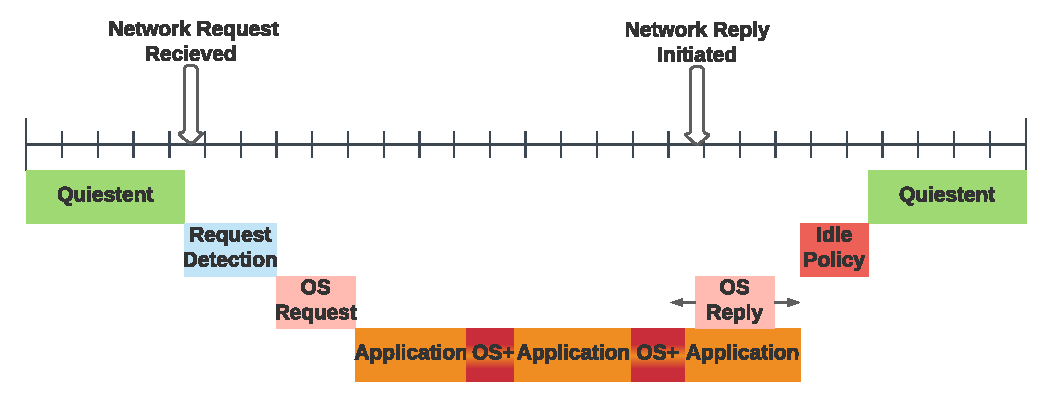
\includegraphics[width=0.5\textwidth]{figures/timeline_chart}
%\caption[]{Logical execution timeline for a single application request}
%\label{fig:timeline}
%\end{figure}

\newpage
%\appendix{\bf{Appendix:}  Mathematical Framework}
\section{\bf{Appendix:}  Mathematical Framework}
\label{sec:appendix}

Under the assumption that the various time-segments in figure~\ref{fig:timeline} don't overlap, one can break down a full cycle from one request to another into disjoint time-intervals:

\begin{equation}
\delta t = t_{\text{detect}} + t_{\text{osreq}} + t_{\text{app}} + t_{\text{idlepolicy}} + t_q = \frac{1}{\lambda}
\label{eq:time}
\end{equation}

where, $\delta t$ = time between the arrivals of two consecutive requests. The other terms represent the various intervals in figure~\ref{fig:timeline}.

Each term is treated as a deterministic and fixed quantity (dependent on workload, hardware, OS, parameters) as opposed to a random variable following some underlying probability distribution. This is sufficient for a qualitative treatment but a full quantitative treatment would treat these terms as part of a probabilistic graphical model.

Note that the interval $\delta t$ is the interarrival time which is given by the reciprocal of the arrival rate (in queries/requests per unit time), $\lambda$. We will work in the regime where $\lambda$ is low enough that each request is processed before the next request arrives. While the treatment above is for the open-loop setting, this restriction also applies to the closed loop setting where, by construction, the interarrival interval always exceeds the time spent processing a request.

To map this timeline decomposition to our experimental setup, we can group together some of the terms to define:

$$t_{\text{work}} = t_{\text{osreq}} + t_{\text{app}} + t_{\text{idlepolicy}}$$

$$t_{\text{latency}} = t_{\text{work}} + t_{\text{detect}}$$

to get:

$$\delta t = t_{\text{detect}} + t_{\text{work}} + t_q = t_{\text{latency}} + t_q$$

Intuitively, $t_{\text{work}}$ is the time spent on processing the request outside the detection phase and outside any quiescent time, $t_q$, and $t_{\text{latency}}$ is the time spent both in the detection phase and on processing for a given request.

Since the total time, $\delta t$ is fixed (=$\frac{1}{\lambda})$, this implies that the quiescent time is,

$$t_q = \left[\frac{1}{\lambda} - (t_\text{work} + t_{\text{detect}})\right]^+$$

where $[x]^+ = \max(x,0)$ i.e. $[x]^+$ is the positive part of $x$. 

In other words, if the arrival rate $\lambda$ is small enough, there is an opportunity for the processor to enter a quiescent state ($t_q > 0$) but as the arrival rate increases, the time processing the request, $t_\text{work}$ exceeds the inter-arrival gap leading to requests accumulating in the queue. 

As stated above, these relationships also applies to the closed-loop case with the additional constraint that the arrival rate and thus the interarrival gap is no longer independent of $t_\text{work}$.

Given this time decomposition, one can compute the total energy consumed for each request as follows:

\begin{equation}
  E = P_\text{detect} t_{\text{detect}} + P_{\text{work}} \left[t_{\text{osref}} + t_{\text{app}} + t_{\text{idlepolicy}}\right] + P_q t_q 
\label{eq:energy}
\end{equation}
The assumption is that there are three power regimes, one each for the detection phase, the work phase and the quiescent phase, respectively.

For the open-loop case, since we are studying energy, $E$ vs latency, $t_{\text{latency}}$ plots for various itr ($t_{detect}$) and DVFS values, we need to posit the dependence of these terms on DVFS. Suppose the workload needs $N_i$ instructions. One would expect $t_\text{work}$ to scale as:

$$t_{\text{work}} \propto \frac{N_i}{f}$$

where f = CPU frequency. Of course, there might be deviations from this behavior and one can posit a power law dependence,

$$t_{\text{work}} = A\frac{N_i}{f^{1+\alpha'}}$$

where A is a constant of proportionality and $\alpha'$ is an arbitrary parameter. $\alpha'$ = 0 would fit the baseline case where time scales inversely with frequency. Since we control DVFS and not frequency directly, we can change this to

$$t_{\text{work}} = A\frac{N_i}{\Delta^{1+\alpha}}$$

where $\Delta$ = the chosen DVFS value and $\alpha$ is some scaling power that can be inferred from data. The other time values don't depend on DVFS in this simple model (although that assumption can be added in a straightforward way).

The total energy consumed depends on various power values which in turn can depend on DVFS. Here, we posit that $P_{\text{work}}$ has a power law dependence on DVFS, $\Delta$. To motivate this, the power consumed by a processor scales as:

$$P \propto V^2 f$$

where V = the operating voltage and f = CPU frequency. DVFS scales both voltage and frequency but not necessarily in a linear way. The general power law assumption is parameterized by a second parameter, $\beta$, as follows:

$$P_{\text{work}} = B \Delta^{2+\beta}$$

where B is a constant of proportionality and $\beta$ can be unrestricted and is meant to be inferred from the data. Depending on the exact setup, it is possible that $P_{\text{detect}}$ also scales with DVFS and in that case, we will set $P_{\text{detect}} = P_{\text{work}}$.

At a qualitative level, the two relationships,

\begin{equation}
    \delta t = t_{\text{detect}} + t_{\text{work}} [=\frac{AN_i}{\Delta^{1+\alpha}}] + t_q
\end{equation}

\begin{equation}
    E = P_\text{detect} t_{\text{detect}} + P_{\text{work}}[=B\Delta^{2+\beta}] t_{\text{work}}[=\frac{AN_i}{\Delta^{1+\alpha}}] + P_q t_q
\end{equation}

with the requirements that $\delta t = \frac{1}{\lambda}$ or equivalently, $t_q = \left[\frac{1}{\lambda} - [t_\text{work}+t_\text{latency}) \right]^+$ can be used to plot the behavior of energy consumed vs time (latency, total run-time) for various values of $\alpha$ and $\beta$.

We can plot some energy, $E$ vs latency, $t_{\text{latency}}$ curves numerically for the case:

$$P_{\text{detect}} = P_q = 0W$$

$$P_{\text{work}} = P_{\text{static}} + P_{text{min}} \Delta^{2+\beta} = 10W + 20W \Delta^{2+\beta}$$

For a fixed interarrival time, $\delta t$, we assign a fraction $f_{\text{detect}}$ to the detection phase and a maximum fraction $f_{\text{work}}^{\text{max}}$ to the work to get:

\begin{equation}
\begin{split}
    t_{\text{latency}} &= t_{\text{detect}} + t_{\text{work}} \\
    &= f_{\text{detect}}\delta t + \frac{f_{\text{work}}^{\text{max}}\delta t}{\Delta^{1+\alpha}}  \\
\implies & \boxed{\frac{t_{\text{latency}}}{\delta t} = f_{\text{detect}} + \frac{f_{\text{work}}^{\text{max}}}{\Delta^{1+\alpha}}}
\end{split}
\end{equation}

and

\begin{equation}
\begin{split}
    E &= P_\text{detect} t_{\text{detect}} + P_{\text{work}}  t_{\text{work}} + P_q t_q \\
    &= P_{\text{work}}  t_{\text{work}} \\
    &= (10W + 20W \Delta^{2+\beta}) (f_{\text{detect}}\delta t + \frac{f_{\text{work}}^{\text{max}}\delta t}{\Delta^{1+\alpha}}) \\
    \implies &\boxed{\frac{E}{1W \delta t} = (10 + 20 \Delta^{2+\beta})(f_{\text{detect}} + \frac{f_{\text{work}}^{\text{max}}}{\Delta^{1+\alpha}})}
\end{split}
\end{equation}

For various choices of detection loads ($0 \leq f_{\text{detect}} \leq 1$), maximal work loads ($0 \leq f_{\text{work}}^{\text{max}} \leq 1$), time-scaling ($\alpha$), power-scaling ($\beta$), we can plot energy (E) vs latency ($t_{\text{latency}}$) curves as DVFS ($\Delta$) varies.

%\subsection{ITR-Delay algorithm}
